\chapter{Sampling Based Inference}
\section{Basic Sampling Methods}
% \subsection{Forward Sampling}

\subsection{Inverse Transform Sampling}
Inverse transform sampling is a basic method for pseudo-random number sampling, \ie for generating sample numbers at random from any probability distribution given its cumulative distribution function (CDF).

\textbf{Assume that we already have a uniformly distributed random number generator}, \eg \textrm{np.random.randn()}
\begin{enumerate}
	\item Generate a random number $u \sim Unif[0,1]$
	\item Find the inverse of the desired CDF, $F_{X}^{-1}(x)$.
	\item Compute $X=F_{X}^{-1}(u)$. The computed random variable $X$ has distribution $F_X(x)$
\end{enumerate}
However, it is \textbf{hard to compute the inverse of CDF} ($F_X(x)$)

	\begin{itemize}
		\item $F_X(x):\mathbb{R}\mapsto [0,1]$ is any CDF. 
		\item CDF is a non-negative and non-decreasing (monotone) function that is continuous. 
		\item Our objective is to simulate a random variable $X$ distributed as $F$; that is, we want to simularte a $X$ such that $P(X\leq x)=F(x)$.
		\item $F$ is invertible since it is continuous and strictly increasing.
%		\item $y$-axis: Uniform distribution
%		\item $x$-axis: sample value
	\end{itemize}

\begin{figure}[t]
	\begin{center}
		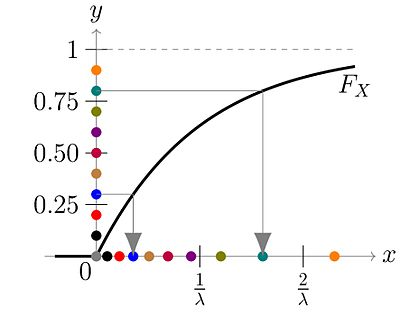
\includegraphics[scale=0.6]{./images/sampling/inverse.jpg}
	\end{center}
	\caption{$y$-axis: Uniform distribution, $x$-axis: sample value}
\end{figure}

\begin{figure}[t]
	\begin{center}
		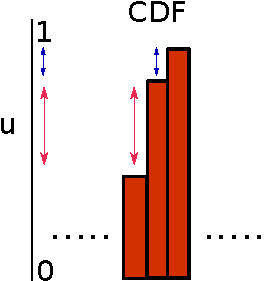
\includegraphics[scale=1.2]{./images/sampling/cdf.pdf}
	\end{center}
	\caption{How can this sampling method recover the original distribution?}
\end{figure}

\subsection{Ancestral Sampling}
$$p(\mathbf{x}) = p(\mathbf{x}_1)p(\mathbf{x}_2|\mathbf{x}_1)p(\mathbf{x}_3|\mathbf{x}_2)\cdots$$
Sampling steps:
\begin{enumerate}
	\item sample $\mathbf{x}_1$
	\item sample $\mathbf{x}_2$ conditioned by $\mathbf{x}_1$
	\item sample $\mathbf{x}_3$ conditioned by $\mathbf{x}_2$
\end{enumerate}



\subsection{Rejection Sampling}
Rejection sampling is a simple method. It rejects samples violating a given condition (\eg conditions of conditional probability.). Let's see its theory. 

Rejection sampling is a method for sampling from a distribution $p(x)=\frac{1}{Z}p'(x)$ that is difficulut to sample directly, but its unnormalized pdf $p'(x)$ is east to evaluate ($Z$ is hard to compute). In rejection sampling, we need some simpler distribution $q(x)$, called a \textbf{proposal distribution}. 

The intuition of rejection sampling is actually similar to Monte-Carlo estimation. By setting a large area (proposal distribution), we can sample points and take them that are inside the our target distribution

% The $k$ must be sufficiently large to envelope the true distribution.
To run the rejection sampling, introduce a constant $k$ whose value is chosen such that $kq(x)\geq p'(x)$ for all values of $x$. The function $kq(x)$ is called a comparison function. Each step of the rejection sampler involves generating two random variables:
	\begin{enumerate}
		\item Sample $x_0\sim q$
		\item Sample $u_0\sim U[0,kq(x_0)]$.
	\end{enumerate}
	Finally, If $u_0>p'(x_0)$, then the sample $x_0$ will be rejected, otherwise we add the sample $x_0$ to our set of samples $\{x^{r}\}$.

	\begin{figure}[h]
		\begin{center}
			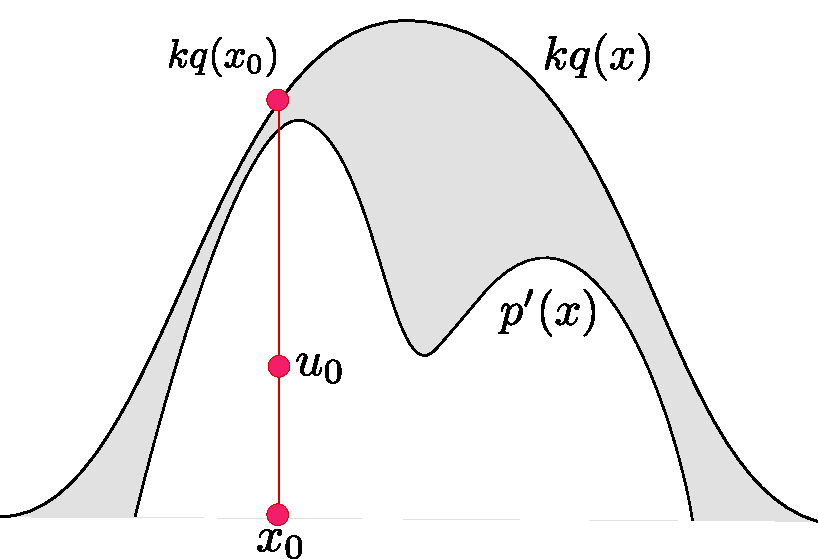
\includegraphics[scale=0.5]{./images/sampling/rejection.pdf}
		\end{center}
	\end{figure}

	The original values of $x$ are generated from the distribution $q(x)$ and these samples are then accepted with probability $p'(x)/kq(x)$ (see the figure above. The acceptance probability (\ie length) is the $p'$ divided by $kq$). Then, the probability that a sample will be accepted is given by   
	\begin{align*}
	p(accept) &= p\Bigg(u\leq \frac{p'(x)}{kq(x)}\Bigg)\\
	&= \int p\Bigg(u\leq \frac{p'(x)}{kq(x)}\bigg|x\Bigg)q(x)dx\\
	% & = \mathbb{E}[p'(x)/kq(x)] \tiny \textrm{ by Lemma 1} \\
	& = \int \frac{p'(x)}{kq(x)}q(x)dx\\
	& = \frac{1}{k}\int p'(x)dx
	\end{align*}
	Thus, the sampling will be more efficient if we choose small $k$ to increase the change of acceptance. 
%	\begin{align*}
%	p(accpet) &= \int p(accpet, x)dx\\
%	& = \int \frac{p'(x)}{kq(x)}q(x)dx\\
%	& = \frac{1}{k}\int p'(x)dx\\
%	& = \frac{1}{k}
%	\end{align*}
%	\begin{align*}
%		p(x^*) &= \frac{[p'(x^*)/kq(x^*)]q(x^*)}{\int [p'(x)/kq(x)]q(x)dx}\\
%		& = \frac{p'(x^*)}{\int p'(x^*)dx}\\
%		& = p(x^*)
%	\end{align*}

\subsection{Importance Sampling}

We want to estimate an expectation of function $f(x), x\sim p(x)$, but it would be hard to estimate the distribution $p(x)$. Again, the importance sampling is not a method for generating samples from $p(\mathbf{x})$. In this case, we can use a simple distribution $q(x)$ by
$$\mathbb{E}(f) = \int f(x)p(x)dx = \int f(x)\frac{p(x)}{q(x)}q(x)dx \approx \frac{1}{N}\sum_{n=1}^N \frac{p(x_i)}{q(x_i)}f(x_i) .$$

%Importance sampling is not a method for generating samples from $p(\mathbf{x})$. It is just a method for estimating the expectation of a function $f(\mathbf{x})$. We first generate $R$ samples $\{x^{(r)}\}$ from $q(x)$, then we could estimate the expectation by Monte Carlo method. However, if the generated samples, values of $x$ where $q(x)$ is greater than $p(x)$ will be over-represented in this estimator, and where $q(x)$ is less than $p(x)$ will be under-represented. Thus, we introduce weights 
%$$w_r = \frac{p(x^*)}{q(x^*)}$$
	
%	%$$\hat{f} = \frac{1}{L}\sum_{l=1}^{L}f(\mathbf{z}^{(l)})$$

\begin{itemize}
	\item Assume that $p(\mathbf{x})$ is known and too complicated to be sampled directly. 
	\item Samples are independently drawn from a \textbf{proposal density} $Q(\mathbf{x})$, which is designed to be close to the true density $p(\mathbf{x})$ and \textbf{simpler}
	\item Generate $R$ samples from $Q(\mathbf{x})$
\end{itemize}
